\documentclass[10pt]{article}
\usepackage[utf8]{inputenc}
\usepackage{url}
\usepackage{hyperref}
\usepackage{amsmath}
\usepackage{amsfonts}
\usepackage{amssymb}
\usepackage{graphicx}
\graphicspath{ {./images/} }
\usepackage{float}
\usepackage{lipsum}
\usepackage{sectsty}
\sectionfont{\centering}
\usepackage{multicol}
\usepackage{xcolor}
\usepackage{natbib}
\usepackage{graphicx}
\usepackage{listings}
\usepackage{xcolor}
\usepackage{pgfplots}
\usepackage[font=small]{caption}
\addtolength{\abovecaptionskip}{-3mm}
\addtolength{\textfloatsep}{-5mm}
\setlength\columnsep{20pt}

\usepackage[a4paper,left=1.50cm, right=1.50cm, top=2cm, bottom=3cm]{geometry}


\author{}

\title{\Large{Design and Analysis of Algorithms Assignment - 5}}

\begin{document}

	\begin{center}
		{\Large \textbf{Design and Analysis of Algorithms Assignment - 5}}\\
		\vspace{1em}
		{\large Department of Information Technology,}\\
		\vspace{1em}
		\large{Indian Institute of Information Technology, Allahabad 211015, India}\\
		\vspace{1em}
		\large{SUBHASH BALLA(IIT2019207), DHANUSH VASA (IIT2019208)}
		\vspace{2.5em}

	\end{center}

%\begin{multicols*}{2}
\iffalse
    \textbf{\emph{{Abstract}: The problem is to find out the two polynomials represented by two arrays of a function.   In  this  paper,  this  triv-ial  problem  of  finding  that multiplies given two polynomials  has  been  solved  using  thetechniques  and  ideas  based  on  Divide  and  Con-quer  Programming  Paradigm.   Also,  this  paperdiscuss  the  distance  between  these  polynomials of two arrays also.   Using  the  Divide  and  Conquerapproach,  the  algorithm  achieves  its  best  timecomplexity of O(n),thus reducing the time toa  much  significant  extent.  Thus  the  approach  ofDivide and Conquer exhibits the logarithmic timeand speeds up the mechanism of finding the multiples of given two polinomials.this divide and conquer algorithm recursively breaks down a problem into two or more sub problems.}}\\

	\textbf{\emph{{Index Terms}: Arrays, Divide and Conquer, Merge Sort, Sorting , Points\\}}
\fi

\section*{INTRODUCTION}

Given a matrix a size n times m,the task is to find maximum length snake sequence and print any of the sequence with maximum length.Also there are some conditions that need to be obeyed for a sequence to be a snake sequence.
This problem is to be done with dynamic programming paradigm.\\\\
\textbf{Dynamic Programming} -  This algorithmic technique can be used to solve problems of types-\\\\
1)optimisation problems(our problem is of this type)\\
2)decision problems\\
3)counting no.of ways\\

We can think of it as a careful brute force approach.we will iterate over all possible solutions and choose the best  solution similar to naive algorithm,but once we find a solution to a sub problem(of course of similar type as actual problem),we store it in memory so that whenever we required that solution,need not compute it again.\\

This can greatly influence the run time of our algorithm.A lot of algorithmic problems which runs in exponential time when implemented naively can be run in polynomial time with dynamic programming paradigm


\iffalse
  The problem is to find out the product of two polynomials.Divide and conquer paradigm is used to solve this task.we will see that run time of this algorithm based on divide and conquer approach is efficient compared to the naive algorithm.Usually the  approach  of Divide and Conquer exhibits the logarithmic time.Divide and conquer algorithm recursively breaks down a problem into two or more sub problems of the same type.

\begin{enumerate}
    \item\textbf{Divide:} Breaking the problems into subproblems of same type.
    \item\textbf{Conquer:} Recursively solve these subproblems.this step receives a lot of smaller sub problems to be solved.
    \item\textbf{Combine:} appropriately combine the answers.When the smaller sub-problems are solved,this stage recursively combines them until they formulate solution of the original problem.\\\\
\end{enumerate}



\paragraph{Advantages of Divide and Conquer}
The advantages of using Divide and conquer algorithm reflects in time and space complexity tremendously than using all the brute force approaches.\\

\textbf{Time Efficiency}\\Complexity of Brute Force is in general high order in nature.We will see that divide and conquer based algorithm reduces the run time from O(n^{2}) to  O(n^{\log _2 3}).\\\\


\textbf{Space Efficiency:} The space complexity of an algorithm or a computer program is the amount of memory space required to solve an instance of the computational problem as a function of characteristics of the input. It is the memory required by an algorithm until it executes completely which are based on the recursive algorithms generally tend to occupy more space in internal allotted stack of the process in RAM(Random Access Memory).Note that, There are methods to do multiplication faster than O(n^2) time.
\fi

\section*{ALGORITHM DESIGN}
Given a  matrix  a[][] of size n*m.\\
Define dp[][] of size n*m where,\\\\
   \textbf{ dp[i][j] stores maximum snake sequence length starting at (i,j).}\\\\
    From the question,it is clear that a snake starting at a a position (say (i,j)) can only move right or down.\\\\
  We will traverse dp array in such a a way that  while we are at position (i,j),we would have already calculated dp(i,j+1) and dp(i+1,j).It's because that dp(i,j) requires dp(i+1,j) and  dp(i,j+1).\\
 One possibility is to  traverse from bottom-right to top-left.\\\\
\textbf{ conditions} - \\
 we can move from \\
       \[ (i,j)  -> (i,j+1) <=>  a[i][j]-a[i][j+1]=(+|-)1\]
      \[(i,j)  -> (i+1,j)  <=> a[i][j]-a[i+1][j]=(+|-)1\]
   \textbf{Possibiltites }-\\\\
 1)  (!right possible AND !down possible), dp[i][j]= 1  ( snake starts and ends at (i,j))\\
 2) (right possible AND down possible),   dp[i][j]= 1+max(dp[i][j+1],dp[i+1][j])\\
 3) (right possible AND  !down possible),  dp[i][j]=1+dp[i][j+1]\\
 4) (!right possible AND  down possible),  dp[i][j]=1+dp[i+1][j]\\

   \textbf{Base cases} -\\\\
   dp[n][m]=1  (no more cells right or down of (n,m)).\\
    right most column  -  snake can only go down.\\
    bottom most row  -  snake can only go right.\\

   \textbf{ Final Answer} -\\\\
                   \textbf{ max\{dp[i][j]\}} \(\forall\)   \(   1<=i<=n\) , \(1<=j<=m\)\\

  \textbf{Trace path} - \\\\
    To trace the path of maximum snake sequence,\\
    we maintain a matrix \textbf{path[][]}   where\textbf{ path[i][j]} points to either \textbf{RIGHT} or \textbf{DOWN} cell(which ever of dp(i+1,j) ,dp(i,j+1) yields maximum) or \textbf{NONE },if it has to end there it self.\\

\iffalse
\paragraph{Data Structures Used:}

\begin{itemize}

\item	Arrays to store the set of polynomials and their result.\\
\end{itemize}
Assume both A(x),B(x) polynomials are of degree n.



\paragraph{Algorithmic Steps:}

The approach based on Divide and Conquer technique of finding the result of multiplying 2 polynomials together. Following is the algorithmic procedure:
\begin{enumerate}

\item	The sizes of the two polynomials is created randomly by rand() number generator function.
\item	The input of the arrays which stores the polynomials data is again created by the rand() number generator.
\item	Here we send these two arrays into the function polymult where it multiplies the two polynomial.
\item	In the function polymult() it creates multiple vector arrays which will store the final results of each component of the resulting polynomial.
\item	Next divides the polynomial stored arrays into two halves. Which is Divide and Conquer algorithm.
\item	Then sends these split polynomials again the function polymult again in a recursive manner.
\item	 Followed by sending the results of polymult in to the polyadd functions which adds the results in multiplication manner.
\item As all this is happening the result is stored into the array result.
\end{enumerate}


\paragraph{ATTEMPT 1:}


let,
\[A(x)=a_0+a_1.x+....+a_n.x^n \]  \[and\]   \[B(x)=b_0+b_1.x+...+b_n.x^n\]
Define
\[A_0(x)=a_0+a_1.x+  ....  +a_{[n/2]-1}.x^{[n/2]-1}\]
\[A_1(x)=a_{[n/2]}+a_{[n/2]+1}.x+  ....  +a_n.x{n-[n/2]}\] where  [.]  is  GIF.\\

Then
\[A(x)=A_0(x)+A_1(x).x^{[n/2]}\]
similarly
\[B(x)=B_0(x)+B_1(x).x^{[n/2]}\]

we have \[A(x).B(x)=A_0.B_0+(A_0.B_1+A_1.B_0).x^{[n/2]}+A_1.B_1.X^{2.[n/2]}\]
we can see that original problem of size n is divided into 4 sub problems  of degree n/2.\[ (i.e; computing  A_0B_0 , A_0B_1 , A_1B_0 , A_1B_1)\]
After computing them,we simply find\\
\[A(x).B(x)=A_0.B_0+(A_0.B_1+A_1.B_0).x^{[n/2]}+A_1.B_1.X^{2.[n/2]}\]
which is simply  polynomial addition (kind of ) and hence takes O(n) time.
so the recurrence we get is \\
\[T(n)=4.T(n/2)+O(n)\]
solving this recurrence, we get \[T(n)=O(n^2)\]
But this is not what we wanted since naive algorithm also works in O(n^2).\\

\paragraph{ATTEMPT 2:}\\
we are computing 4 sub problems.CAN WE DO ANY BETTER?\\
consider ,\\
\[X=A_0.B_0\]
\[Y=A_1.B_1\]
\[Z=(A_0+A_1).(B_0+B_1)\]
required is\[ (A_0.B_1+A_1.B_0)=Z-X-Y\]
hence,by only computing 3 sub problems (X,Y,Z) we can get \\
\[A(x).B(x)=X+(Z-X-Y).X^{[n/2]}+Y.x^{2.[n/2]}\]
the recurrence relation(discussed in analysis part) what we get now is ,\\
\[T(n)=3.T(n/2)+O(n)\]
solving this recurrence,we get
\[T(n)=O(n^{log_2 3})=O(n^{1.585})\]
which is obviously better than O(n^2).
\fi

\lstset { %
    language=C++,
    backgroundcolor=\color{black!5},
    basicstyle=\footnotesize,
}
\section*{Code Implementation}
\lstset { %
    language=C++,
    backgroundcolor=\color{black!5},
    basicstyle=\footnotesize,
}
\begin{lstlisting}

#include<bits/stdc++.h>
using namespace std;
#define IOS ios_base::sync_with_stdio(false),cin.tie(NULL)
#define mod 1000000007
#define  pb push_back
typedef long long ll;
typedef unsigned long long ull;
typedef  long double ld;
typedef vector<int> vi;
typedef vector<bool> vb;
typedef vector<vi >vvi;
typedef vector<ll> vll;
typedef vector<vll >vvll;


ll n, m;
ll maxN = 101, maxnumber = 5;
ll pos_i = 1, pos_j = 1, max_length = 1;
ll a[1001][1001], dp[1001][1001];
ll path[1001][1001], path_table[1001][1001];


void print_path() {


	while (true) {
		path_table[pos_i][pos_j] = a[pos_i][pos_j];
		if (path[pos_i][pos_j] == 1)pos_j++;
		else if (path[pos_i][pos_j] == -1)pos_i++;
		else break;
	}

	for (ll i = 1; i <= n; i++) {
		for (ll j = 1; j <= m; j++)cout << path_table[i][j] << " ";
		cout << "\n";
	}
}


void solve() {


//base_cases---->

	dp[n][m] = 1;
	path[n][m] = 0;


//bottom most row
	for (ll i = m - 1; i >= 1; i--) {
		if (a[n][i] == a[n][i + 1] + 1 || a[n][i] == a[n][i + 1] - 1) {
			dp[n][i] = dp[n][i + 1] + 1, path[n][i] = 1;
			if (dp[n][i] > max_length)max_length = dp[n][i], pos_i = n, pos_j = i;
		}
		else dp[n][i] = 1;
	}


//right most coulmn
	for (ll i = n - 1; i >= 1; i--) {
		if (a[i][m] == a[i + 1][m] + 1 || a[i][m] == a[i + 1][m] - 1) {
			dp[i][m] = dp[i + 1][m] + 1, path[i][m] = -1;
			if (dp[i][m] > max_length)max_length = dp[i][m], pos_i = i, pos_j = m;
		}
		else dp[i][m] = 1;
	}



for (ll i = n - 1; i >= 1; i--) {
	for (ll j = m - 1; j >= 1; j--) {

  bool right_possible = false, down_possible = false;

 if (a[i][j] == a[i][j + 1] + 1 || a[i][j] == a[i][j + 1] - 1)right_possible = true;
 if (a[i][j] == a[i + 1][j] + 1 || a[i][j] == a[i + 1][j] - 1)down_possible = true;

if (!right_possible && !down_possible) {
			dp[i][j] = 1;
			continue;
 }

if (right_possible)dp[i][j] = dp[i][j + 1] + 1, path[i][j] = 1;

if (down_possible && dp[i + 1][j] + 1 > dp[i][j])dp[i][j] = dp[i + 1][j] + 1, path[i][j] = -1;

if (dp[i][j] > max_length)max_length = dp[i][j], pos_i = i, pos_j = j;
		}
	}

cout << "maximum length is----> " << max_length << "\n";
cout << "path--->\n";
print_path();
}

int main() {

IOS;
srand(time(0));

n = rand() % maxN + 1, m = rand() % maxN + 1;

cout << "matrix width and height are--> \n" << n << " " << m << "\n";

for (ll i = 1; i <= n; i++)for (ll j = 1; j <= m; j++)a[i][j] = rand() % maxnumber + 1;

cout << "\ninput matrix is---> \n";
	for (ll i = 1; i <= n; i++) {
		for (ll j = 1; j <= m; j++)cout << a[i][j] << " ";
		cout << "\n";
	}

solve();
}

\end{lstlisting}


\iffalse
\begin{lstlisting}

#include<bits/stdc++.h>
using namespace std;
#define mod 1000000007
#define  pb push_back
typedef long long ll;
typedef unsigned long long ull;
typedef  long double ld;
typedef vector<int> vi;
typedef vector<bool> vb;
typedef vector<vi >vvi;
typedef vector<ll> vll;
typedef vector<vll >vvll;

ll n, m;
ll maximumdegree,large_num=1000000;
vll result(10001), a(10001), b(10001);



void print_poly(vll& a, ll deg) {

	for (ll i = 0; i < deg; i++)cout << a[i]
	<< "*x^" << i << "+ ";
	cout << a[deg] << "*x^" << deg << "\n";
}

void build_poly(vll& a,ll st,ll en,vll& result){

	for (ll i = st; i <= st + en; i++)
	result[i - st] = a[i];
}

void poly_add(vll& a,vll& b,ll deg,ll bias1,
ll bias2,vll& result){

for (ll i = 0; i <= deg; i++)
result[i] = (i - bias1 >= 0 ? a[i - bias1] : 0)
	+ (i - bias2 >= 0 ? b[i - bias2] : 0);
}

void self_sub(vll& a, vll& b, ll deg) {

for (ll i = 0; i <= deg; i++)a[i] -= b[i];
}

void poly_mult(vll& a,vll& b,ll deg,vll& result)
{

vll a0(2 * deg + 1), a1(2 * deg + 1);
vll b0(2 * deg + 1), b1(2 * deg + 1);
vll a0b0(2 * deg + 1), a1b1(2 * deg + 1);
vll a0a1(2 * deg + 1), b0b1(2 * deg + 1);
vll a0b1_a1b0(2 * deg + 1);

if (deg == 0 || deg == 1) {
	if (deg == 0)result[0] = a[0] * b[0];
	else
	result[0] = a[0] * b[0];
	result[1] = a[0] * b[1] + a[1] * b[0];
	result[2] = a[1] * b[1];
		return;
	}

ll deg_0 = deg / 2 - 1, deg_1 = deg - deg / 2;

build_poly(a, 0, deg_0, a0);
build_poly(b, 0, deg_0, b0);
build_poly(a, deg_0 + 1, deg_1, a1);
build_poly(b, deg_0 + 1, deg_1, b1);
poly_mult(a0, b0, deg_0, a0b0);
poly_mult(a1, b1, deg_1, a1b1);
poly_add(a0, a1, max(deg_0, deg_1), 0, 0, a0a1);
poly_add(b0, b1, max(deg_0, deg_1), 0, 0, b0b1);
poly_mult(a0a1, b0b1, max(deg_0, deg_1), a0b1_a1b0);
self_sub(a0b1_a1b0, a0b0, deg);
self_sub(a0b1_a1b0, a1b1, deg);
poly_add(a0b0,a0b1_a1b0,2ll*deg,0,deg/2,result);
poly_add(result,a1b1,2ll*deg,0,2ll*(deg/2),result);
}



int main() {

	cin >> n >> m;
	for (ll i = 0; i <= n; i++)cin >> a[i];
	for (ll i = 0; i <= m; i++)cin >> b[i];
	cout << "a_polyomial is--->\n";
	print_poly(a, n);
	cout << "b_polynomial is--->\n";
	print_poly(b, m);

	poly_mult(a, b, max(n, m), result);

	cout << "resultant polynomial is--->\n";
	print_poly(result, n * m + 1);
}

\end{lstlisting}
\begin{lstlisting}
#include<bits/stdc++.h>
using namespace std;
#define IOS ios_base::sync_with_stdio(false),cin.tie(NULL)
#define mod 1000000007
#define  pb push_back
typedef long long ll;
typedef unsigned long long ull;
typedef  long double ld;
typedef vector<int> vi;
typedef vector<bool> vb;
typedef vector<vi >vvi;
typedef vector<ll> vll;
typedef vector<vll >vvll;

ll n, m;
ll maximumdegree=10,large_num=1000000;
vll result(1111111), a(1001), b(1001);



void print_poly(vll& a, ll deg) {

	for (ll i = 0; i < deg; i++)cout << a[i] << "*x^" << i << "+ ";
	cout << a[deg] << "*x^" << deg << "\n";
}

void build_poly(vll& a, ll st, ll en, vll& result) {

	for (ll i = st; i <= st + en; i++)result[i - st] = a[i];
}

void poly_add(vll& a, vll& b, ll deg, ll bias1, ll bias2, vll& result) {

	for (ll i = 0; i <= deg; i++) {
		result[i] = (i - bias1 >= 0 ? a[i - bias1] : 0) +
                          (i - bias2 >= 0 ? b[i - bias2] : 0);
	}

}

void self_sub(vll& a, vll& b, ll deg) {

	for (ll i = 0; i <= deg; i++)a[i] -= b[i];
}

void poly_mult(vll& a, vll& b, ll deg, vll& result) {

    	vll a0(2 * deg + 1), a1(2 * deg + 1);
        vll b0(2 * deg + 1), b1(2 * deg + 1);
        vll  a0b0(2 * deg + 1), a1b1(2 * deg + 1);
        vll  a0a1(2 * deg + 1), b0b1(2 * deg + 1);
        vll  a0b1_a1b0(2 * deg + 1);



	//base cases-->
	if (deg == 0 || deg == 1) {
		if (deg == 0)result[0] = a[0] * b[0];
		else{
			result[0] = a[0] * b[0];
            result[1] = a[0] * b[1] + a[1] * b[0];
            result[2] = a[1] * b[1];
            }
		return;
	}

	ll deg_0 = deg / 2 - 1, deg_1 = deg - deg / 2;

    build_poly(a, 0, deg_0, a0);
    build_poly(b, 0, deg_0, b0);
    build_poly(a, deg_0 + 1, deg_1, a1);
    build_poly(b, deg_0 + 1, deg_1, b1);

	poly_mult(a0, b0, deg_0, a0b0);
	poly_mult(a1, b1, deg_1, a1b1);
	poly_add(a0, a1, max(deg_0, deg_1), 0, 0, a0a1);
    poly_add(b0, b1, max(deg_0, deg_1), 0, 0, b0b1);
	poly_mult(a0a1, b0b1, max(deg_0, deg_1), a0b1_a1b0);
	self_sub(a0b1_a1b0, a0b0, deg);
    self_sub(a0b1_a1b0, a1b1, deg);
	poly_add(a0b0, a0b1_a1b0, 2ll * deg, 0, deg / 2, result);
	poly_add(result, a1b1, 2ll * deg, 0, 2ll * (deg / 2), result);

}



int main() {
	IOS;
	srand(time(0));

	n = rand() % maximumdegree + 1, m = rand() % maximumdegree + 1;

	for (ll i = 0; i <= n; i++)a[i] = rand() % large_num + 1 ;
	for (ll i = 0; i <= m; i++)b[i] = rand() % large_num + 1;

	cout << "a_polyomial is--->\n"; print_poly(a, n);
	cout << "\n";
	cout << "b_polynomial is--->\n"; print_poly(b, m);
	cout << "\n";

	poly_mult(a, b, max(n, m), result);

	cout << "resultant polynomial is--->\n";
	print_poly(result, n * m + 1);
}
\end{lstlisting}
\fi


\section*{ALGORITHM ANALYSIS}

%\paragraph{time complexity:}\\
\rule{9cm}{1pt}\\
{
    Number of sub problems=\textbf{n*m.}\\
    Time per subproblem=\textbf{O(1)} (only finding maximum of 2 values).\\
    Hence \textbf{T(n,m)=(n*m)*O(1).}\\
                           =\textbf{O(n*m)\\\\}
    We have created \textbf{dp[][]} and \textbf{path[][]}  of n*m size.\\
    Hence \textbf{auxillary space=O(n*m)}\\\\
    However,If we don't want to trace the path and our only objective is to find maximum snake sequence length,then we can optimise space to \textbf{O(m)}.Its because that that only (i+1)th row is sufficient to clalculate ith row.


 }
\rule{9cm}{1pt}

 \section{Experimental Analysis}
In the following table some cases are plotted for the first algorithm,\newline
\begin{center}
 \begin{tabular}{||c | c | c||}
 \hline
 m & n & Time Taken (in ms) \\ [0.5ex]
 \hline\hline
 10 & 10 & 0.0000 \\
 \hline
 50 & 50 & 0.0000 \\
 \hline
 100 & 100 & 0.0000 \\
 \hline
 500 & 500 & 0.0500 \\
 \hline
 700 & 700 & 0.0600 \\
 \hline
 800 & 800 & 0.0700 \\
 \hline
 900 & 900 & 0.1200 \\
 \hline
 1000 & 1000 & 0.1400 \\
 \hline
 2000 & 2000 & 0.4800 \\
 \hline
 5000 & 5000 & 2.2800 \\ [1ex]
 \hline
\end{tabular}
\end{center}

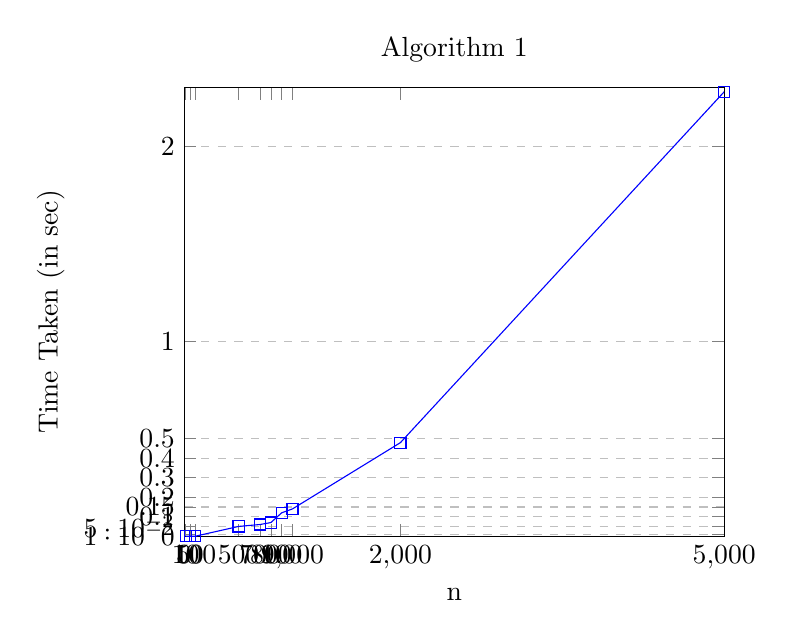
\begin{tikzpicture}
\begin{axis}[
    title={Algorithm 1},
    xlabel={n},
    ylabel={Time Taken (in sec)},
    xmin=0, xmax=5000,
    ymin=0, ymax=2.3000,
    xtick={0,10,50,100,500,700,800,900,1000,2000,5000},
    ytick={0,0.0100, 0.0500, 0.1000, 0.1500, 0.2000, 0.3000,0.4000,0.5000,1.0000,2.000,2.5000},
    legend pos=north west,
    ymajorgrids=true,
    grid style=dashed,
]

\addplot[
    color=blue,
    mark=square,
    ]
    coordinates {
    (10,0.0000)(50,0.0000)(100,0.0000)(500,0.0500)(700,0.0600)(800,0.0700)(900,0.1200)(1000,0.1400)(2000,0.4800)(5000,2.2800)
    };

\end{axis}
\end{tikzpicture}\newline


\iffalse
\section*{APPLICATIONS}
Divide and Conquer is a wide variety of algorithmic technique which solves difficult problems with ease.these are efficient when compared with counterpart brute-force approach.it do not needs any modifications .this strategy uses recursion that makes it a little slower. Some of the applications of the Divide and Conquer Approach are:

\begin{enumerate}
\item \textbf{Merge Sort}
\item \textbf{Quick Sort}
\item \textbf{Binary Search}
\item \textbf{Segment Trees}
\item  \textbf{Strassen’s Algorithm} etc many more.\fi
\end{enumerate}

\section*{CONCLUSION}

We can conclude that the given problem of finding maximum length snake sequence and tracing the path is acheieving the time and space complexities of \textbf{O(n*m)}.

\section*{ACKNOWLEDGMENT}

We are very much grateful to our Course instructor Mr.Rahul Kala and our mentor, Ms.Tejasvee, who have provided the great opportunity to do this wonderful work on the subject of Design and Analysis of Algorithms, specifically on the algorithmic  paradigm of Dynamic Programming.

\section*{NOTE}
1)One can adjust the maximum values of n and m by changing \textbf{maxN } and matrix elements with \textbf{maxnumber}  variables which are declared  as global variables.\\
2)The submitted code contains comments.One can check what's happening at each step.


\section*{REFERENCES}

\begin{enumerate}
\item Introduction to Algorithms by Cormen,Charles, Rivest and Stein.\\
https://web.ist.utl.pt/~fabio.ferreira/material/asa\\

\end{enumerate}

%\end{multicols*}

\end{document}
